% ------------------------------------------
% habitat count  & fish count 
% ------------------------------------------

\subsection{Habitat characteristics and preferences}

To answer the question if different species or genera of weakly electric fish prefer different habitat characteristics, weakly electric fish were recorded in a network of river channels in the LLanos of the Orinoco basin, Meta, Colombia. For each recording the microhabitat's characteristics were categorised. In total, within 13 larger habitats, 139 microhabitat's characteristics, such as the presence or absence of stones, sand, mud, roots and plants, were denoted.\\
Within most (115~microhabitats, 83~\%) of the examined microhabitats stones were frequently found on the ground (fig.~\ref{fig:habitat_count}). In 47 microhabitats  (34~\%) the stream bed was additionally or solely covered with sand. Roots were often (62~microhabitats,~45~\%) found on the shoreline, on the ground or as locked driftwood. Both, mud (7~microhabitats,~5~\%) and plants (14~microhabitats,~10~\%), were clearly less frequent than other examined characteristics.\\
For each microhabitat the species or genus of each recorded fish was determined. Over all, 327 weakly electric fish were recorded. \textit{Apteronotus} was by far the most frequent species. Approximately 250 of the recorded animals (76~\%) were identified as \textit{Apteronotus macrostomus} (fig.~\ref{fig:fish_count_eod}~A). The EOD frequency of these animals ranged from approximately 560~to 1000~Hz and was slightly trimodal distributed (fig.~\ref{fig:fish_count_eod}~B). About 50 fish (15~\%) were identified as \textit{Eigenmannia virescens}. Their EODf mainly varied from 290~to 600~Hz. With 20~(6~\%) recorded individuals pulsefish were by far the least frequent. The EODf of this genus is less than 100~Hz.

\begin{figure}[H]
    \centering
    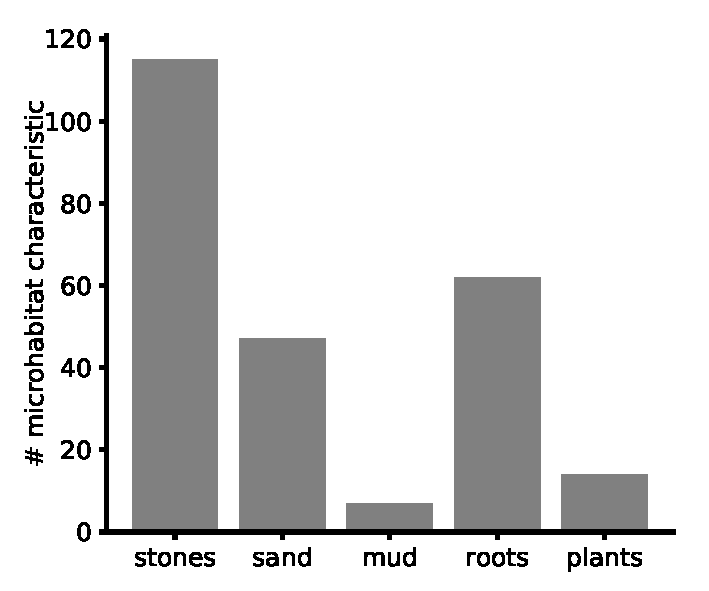
\includegraphics[width=0.7\textwidth]{pictures/Results/JULE_habitat_ccharacteristics.pdf}
    \caption{\textbf{Habitat characteristics.} Total count of the different microhabitat characteristics: stones, sand, mud, roots or different kinds of plants. A single microhabitat could consist of multiple of these categories. Over-all, 139 microhabitats were characterised.}
    \label{fig:habitat_count}
\end{figure}

\begin{figure}[H]
    \centering
    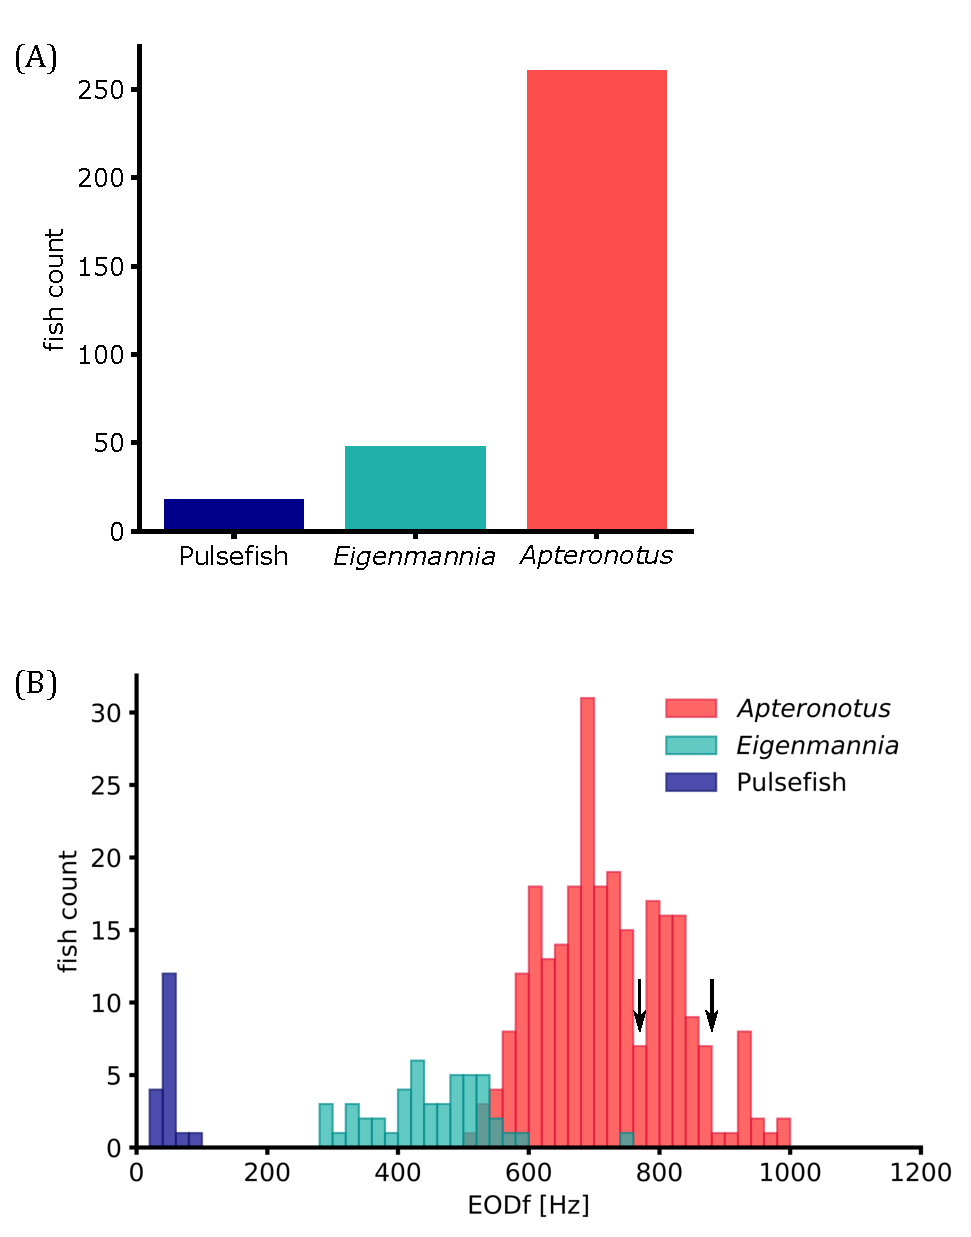
\includegraphics[width=0.9\textwidth]{pictures/Results/fish_count_EOD.pdf}
    \caption{\textbf{Proportion of fish species and EOD distribution.} \textbf{A:}~Shown is the number of animals that were recorded within the 139 investigated microhabitats for each species (\textit{Apteronotus macrostomus} and \textit{Eigenmannia virescens}) or genus (pulsefish). \textbf{B:}~Distribution of the EOD frequencies (EODf) for each species or genus. In case of \textit{Apteronotus}, the first arrow (762~Hz) indicates the border between female and male individuals. The second arrow (880~Hz) marks the border between males with lower EODf (lower dominance) and higher EODf (highly dominant males).}
    \label{fig:fish_count_eod}
\end{figure}

% ---------------------------------------------
% species and habitats
% ---------------------------------------------

Regarding the average fish count dependent on the microhabitat characteristics, some differences between the different species or genera can be seen, especially regarding \textit{Apteronotus} (fig.~\ref{fig:habitat_count_species}). On average, in each microhabitat containing stones, two \textit{Apteronoti} were found. Close to roots on average only one \textit{Apteronotus} was found. In microhabitats with sand, mud and plants, this species was less frequent.
Most \textit{Eigenmannia}s were found in habitats with roots. On average the probability of finding an \textit{Eigenmannia} within a microhabitat with roots was 75~\%. The probability of finding an individual of this species within a stony, sandy or muddy habitat reached from 25~to 50~\%. Not a single animal was found in a microhabitat containing plants.
In contrast, most of the pulsefish, with a probability of 70~\%, were found in habitats with plants. The probability of finding a pulse-type fish within a microhabitat containing sand, mud or roots ranged between 25~and 50~\%. Pulsefish were the less frequent in stony habitats.

\begin{figure}[H]
    \centering
    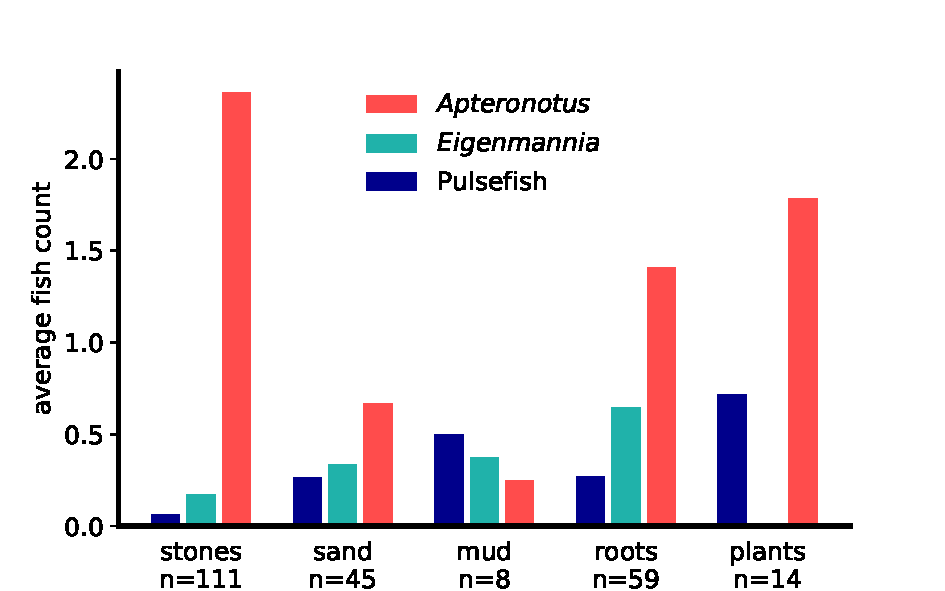
\includegraphics[width = \textwidth]{pictures/Results/average_occuranec_in_habitats.pdf}
    \caption{\textbf{Occurrence of species in the different microhabitats.}
    Shown is the average fish count of Pulsefish (blue), \textit{Eigenmannia virescens} (cyan) and \textit{Apteronotus macrostomus} (red) in an microhabitat with certain characteristics. Microhabitats could contain many different characteristic elements. Hence, a single microhabitat and the corresponding recorded animals can occur more than once in the figure. The average fish count corresponds with the occurrence probability in a microhabitat with a certain characteristic.}
    \label{fig:habitat_count_species}
\end{figure}

\begin{figure}[H]
    \centering
    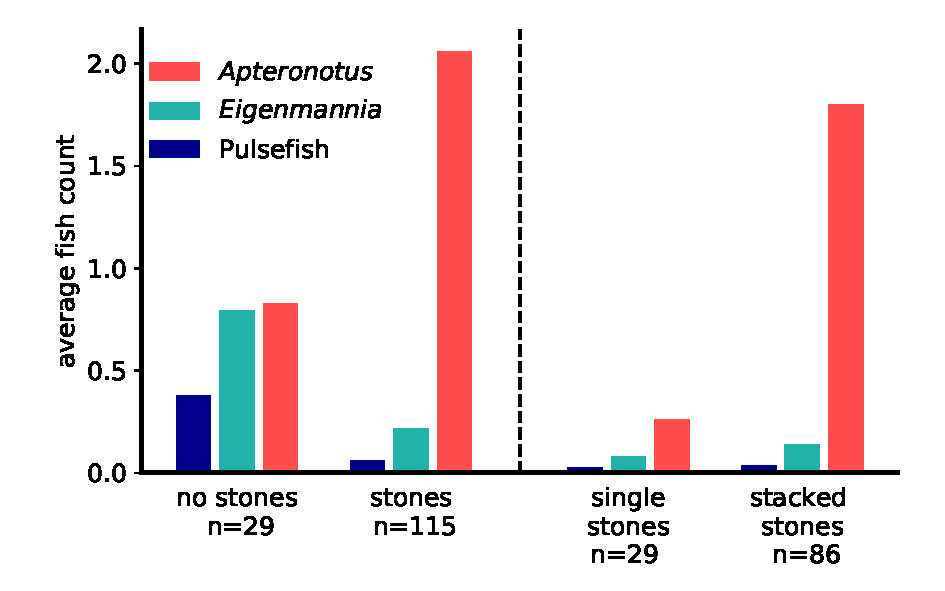
\includegraphics[width = \textwidth]{pictures/Results/more_stones_pls.pdf}
    \caption{\textbf{Occurrence of species in stony habitats.} Shown is the average fish count for Pulsefish (blue), \textit{Eigenmannia virescens} (cyan) and \textit{Apteronotus macrostomus} (red) for microhabitats with and without stones (left). Stony microhabitats are further subdivided into single stones or stacked stones (right). The average fish count corresponds with the occurrence probability in a microhabitat with a certain characteristic.}
    \label{fig:habitat_count_stones}
\end{figure}

Next, we solely looked at the occurrence of the fishes in stony habitats and in habitats without stones (fig.~\ref{fig:habitat_count_stones}). \textit{Eigenmannia} and pulsefish occurred more often in microhabitats without any stones. The probability of finding an individual of the species \textit{Eigenmannia} in a stony microhabitat was 22~\%, for pulsefish 5~\%. Regarding stony habitats, both occurred with the same frequency, regardless whether there were single or stacked stones. Both occurred with a probability of less than 13~\%. In contrast, \textit{A. macrostomus} was clearly more frequent in stony habitats. On average in each stony habitat two individuals of this species were found. In habitats without stones on average only less than one individual was found. A comparison between habitats with single and stacked stones shows, that \textit{Apteronotus} was by far most often found in microhabitats containing stacked stones, with an average fish count of 1,7~individuals per microhabitat.

\begin{figure}[H]
    \centering
    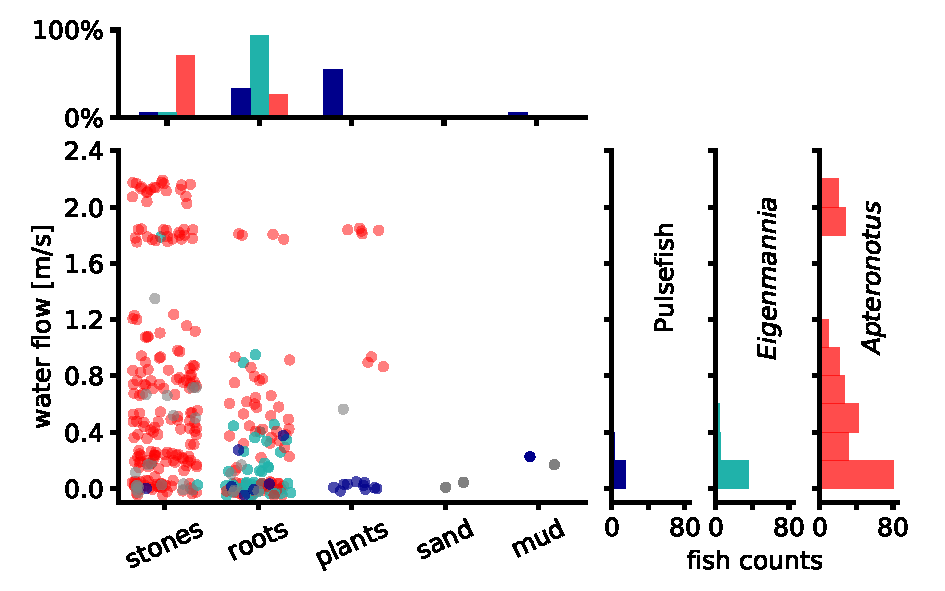
\includegraphics{pictures/Results/flow_habitat_protocol.pdf}
    \caption{\textbf{Distribution of the different fish species over the water flow in different microhabitats.} On the top, for the species \textit{Apteronotus} (red) and \textit{Eigenmannia} (cyan) and the genus of pulsefish (blue) the distribution in the different habitats is shown. The bottom left figure shows the distribution of the fishes in the different habitats over the water flow. The areas with no recorded fish (grey) are shown as well. The habitats are ranked according to the observations in the field. Habitats with roots were ranked above stones, while plants are ranked above roots. If there were neither roots nor plant nor stones, mud was preferred over sand (plants~$>$~roots~$>$~stones~$>$~mud~$>$~sand). The three histograms on the bottom right, show the distribution of the species over the water flow.}
    \label{fig:habitat_vs_flow}
\end{figure}

In contrary to the previous results, in figure~\ref{fig:habitat_vs_flow} every fish is only represented once. Additionally, different microhabitats are ranked based on the observation of the experimenter. The ranking considered that plants are preferred over roots, but if there are no roots and plants, stones were preferred over mud. If there were neither roots, plant, stones nor mud, sandy habitats were occupied (plants~$>$~roots~$>$~stones~$>$~mud~$>$~sand). Mud and sand were considered as less attractive habitats, because they offer less hiding spaces.\\

Besides the ground conditions, the water flow and the water depth were measured in each microhabitat. Comparing the ground conditions and the water flow, a clear difference in occurrence between the species can be seen. Figure~\ref{fig:habitat_vs_flow} shows that pulsefish were found in microhabitats with slow water flow (water flow $<$~0.37~m/s) (median: 0.0~m/s) and preferably in microhabitats with plants, but also in habitats with sand and roots. \textit{Eigenmannia} was also found at lower water speed (median: 0~m/s), mainly in habitats with roots. In contrast, \textit{Apteronotus} was found within a high range of water speed, containing also higher water flows (median: 0.42~m/s). Especially in stony microhabitats, it can be seen that \textit{Apteronotus} rested where the water flow raised up to 2.15~m/s. 
It couldn't be shown, that there was one specific microhabitat were always fish could be found. For each of the researched characteristic there were microhabitats were no fish were found. However, it could be shown that, according to the ranking of microhabitat characteristics, no fish were found in sand.

\begin{figure}[H]
    \centering
    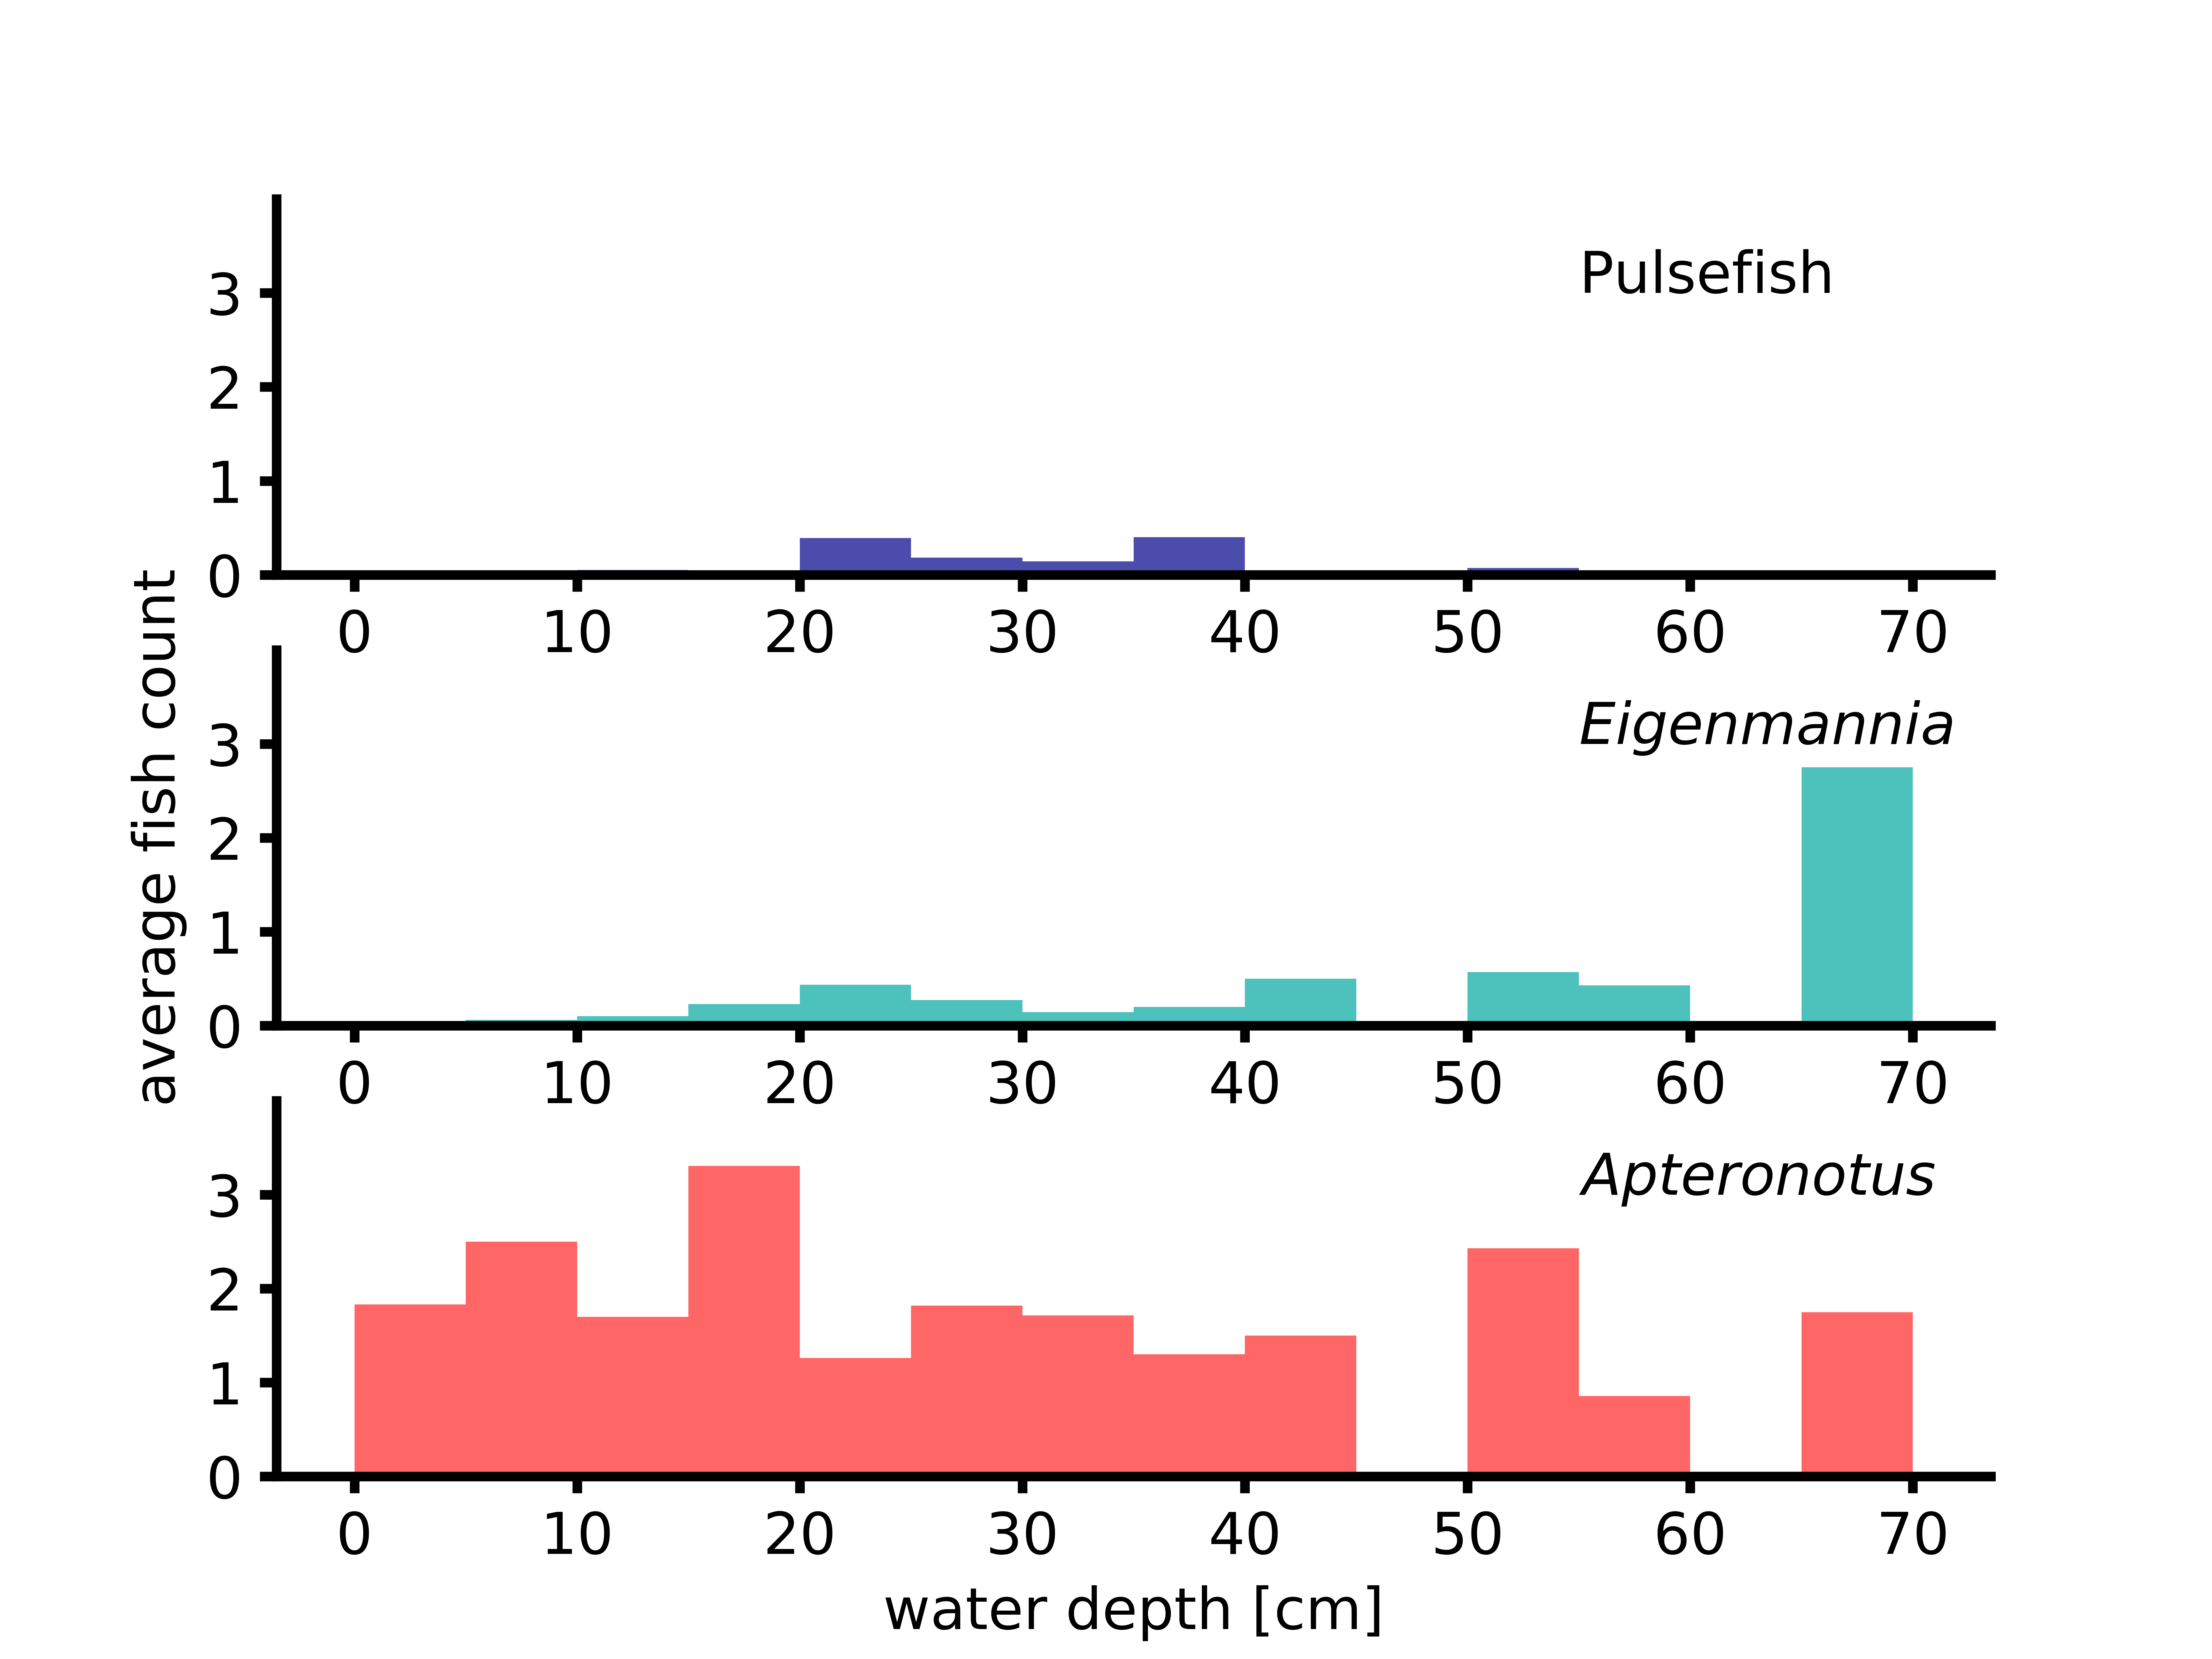
\includegraphics[width=0.9\textwidth]{pictures/Results/JULE_flow_depth2.png}
    \caption{\textbf{Occurrence of species dependent on water depth.} Shown is the average fish count for microhabitats within a certain range of water depth for pulsefish (blue), \textit{Apteronotus macrostomus} (red) and \textit{Eigenmannia virescens} (cyan). Water depths between 45~and 50~cm and 60~and 65~cm were not measured.}
    \label{fig:habitat_vs_depth}
\end{figure}

In addition to the occurrence of the different species or genera dependent on the water flow, their occurrence dependent on the water depth was investigated. Microhabitats with a water depth of 45~to 50~cm and 60~to 65~cm were not found. Regarding \textit{Apteronotus} and pulsefish, no preference for a certain water depth can be seen (fig.~\ref{fig:habitat_vs_depth}). Pulsefish were found in habitats with a water depth between 10~and 55~cm. \textit{Apteronoti} were found in microhabitats with a water depth ranging from a few centimeters up to 70~cm. Also \textit{Eigenmannia} was found within a large range of water depth (5~to 70~cm). In contrast to the other species or genera, \textit{Eigenmannia virescens} seemed to appear more frequently in habitats with a water depth between 65~and 70~cm.


% ----------------------------------------------
% Apteronoti (male / female) 
% ----------------------------------------------

\subsection{Dominance and habitat preferences in \textit{Apteronotus}}

\begin{figure}[H]
    \centering
    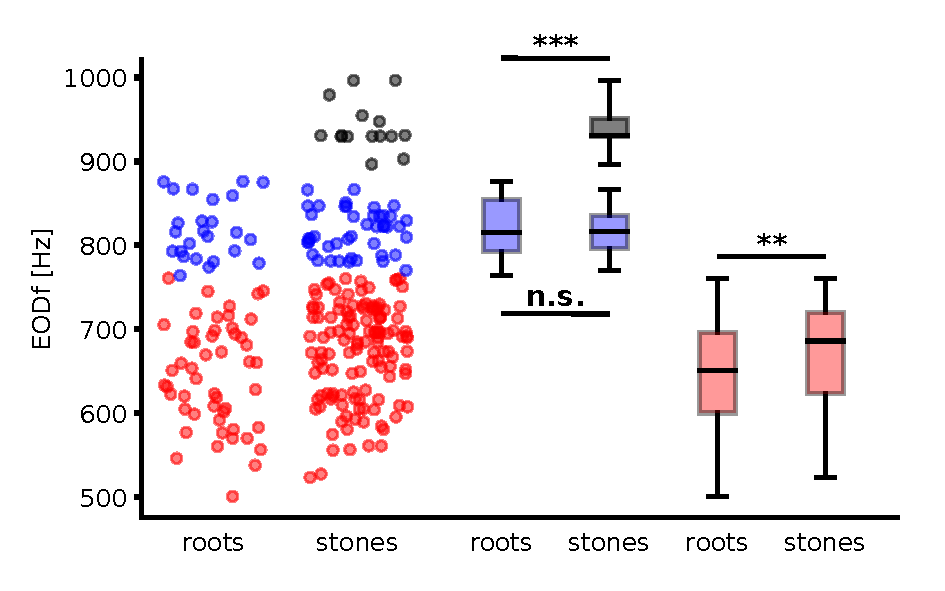
\includegraphics{pictures/Results/eod_habitat.pdf}
    \caption{\textbf{Distribution of the different EODfs of \textit{Apteronotus}, depending on the root and stone microhabitats.} Distribution of male and female \textit{A. macrostomus} in root- and stone-microhabitats. Based on the over-all EOD distribution in figure~\ref{fig:fish_count_eod}, males had an EODf above 762~Hz. The males were also divided into high frequency males and low frequency males at a threshold of 880~Hz.}
    \label{fig:habitat_vs_eod}
\end{figure}

It could be shown that many individuals of the species \textit{Apteronotus macrostomus} occurred in microhabitats made of stones or roots (fig.~\ref{fig:habitat_count_species}). This leads to the question how the different individuals occupy these different microhabitats and if there exists a relation between habitat selection and intra-specific dominance. Since intra-specific dominance is correlated with higher EOD frequencies, the individuals were grouped into three different categories dependent on the EODf: Females, males and high frequency males. According to the EOD frequency distribution in fig.~\ref{fig:fish_count_eod}B and the sexual dimorphism of the EODf, females were defined as having an EODf below 762~Hz. Consequently, recorded males had a EODf above 762~Hz and were further divided into low frequency and high frequency males (EODf~$>$~880~Hz).
Females and males were found in both, stone and root microhabitats (fig.~\ref{fig:habitat_vs_eod}). 
Females in stone and root microhabitats differed in their EOD frequency (Man-Whitney-U-Test: U~=~2385, p~=~0.004, Cohen's~d~=~-0.47). Compared with roots, in stony habitats were more females with higher EODf. The same trend can be seen looking at the males. For the low frequency males, no difference in EODf was found (Man-Whitney-U-Test: U~=~543.5, p~=~0.47). However, the high frequency and hence, the most dominant males, were exclusively found in stony microhabitats.